\section{Prospetto economico}

In questa sezione è presentato il prospetto economico del progetto \ProjectName{}, suddiviso per fasi. Per ogni fase sono indicate le ore preventivate per ogni ruolo impiegato.
Il costo è calcolato utilizzando i dati della tabella al paragrafo \ref{tabellacostiruolo}.

\subsection{Analisi}

A scopo di trasparenza viene redatto il prospetto economico riguardante la fase di Analisi dei requisiti, ma si precisa che le ore spese in questa fase sono a carico del fornitore e non del proponente.

\begin{table}[H]
	\centering
	\begin{tabular}{ l c c }
	\textbf{Ruolo} & \textbf{Ore} & \textbf{Costo} \\
	\hline
	Amministratore & 30 & 600 €\\
	Analista & 58 & 870 €\\
	Progettista & 9 & 198 €\\
	Programmatore & 0 & 0 €\\
	Responsabile & 14 & 420 €\\
	Verificatore & 31 & 465 €\\
	\hline
	\textbf{Totale} & 142 & 2553 €\\
	\hline
	\end{tabular}
	\caption{Ore e costo per ruolo, fase di Analisi}
	\end{table}

I seguenti grafici mostrano il peso orario e di costo di ogni ruolo in questa fase.

\begin{figure}[H]
\centering
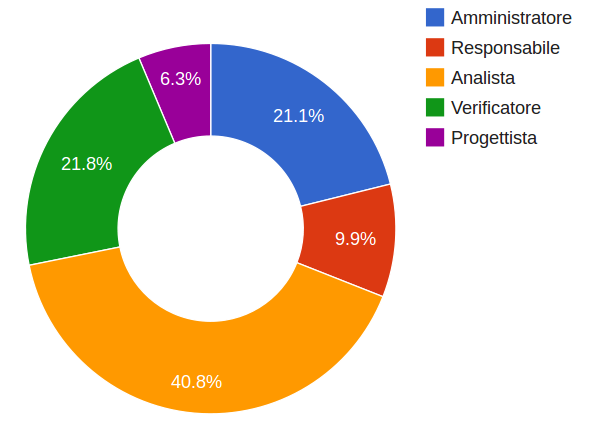
\includegraphics[scale=0.35]{5-1-1.png}
\caption{Ore per ruolo, fase di Analisi\label{fig:nome}}
\end{figure}

\begin{figure}[H]
\centering
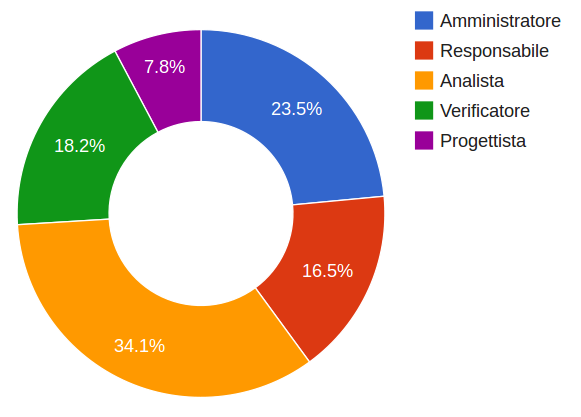
\includegraphics[scale=0.35]{5-1-2.png}
\caption{Costo per ruolo, fase di Analisi\label{fig:nome}}
\end{figure}

\subsection{Progettazione architetturale}

Nella fase di Progettazione architetturale le ore per ogni ruolo sono state cosi suddivise:

\begin{table}[H]
	\centering
	\begin{tabular}{ l c c }
	\textbf{Ruolo} & \textbf{Ore} & \textbf{Costo} \\
	\hline
	Amministratore & 14 & 280 €\\
	Analista & 0 & 0 €\\
	Progettista & 133 & 2926 €\\
	Programmatore & 0 & 0 €\\
	Responsabile & 3 & 90 €\\
	Verificatore & 49 & 735 €\\
	\hline
	\textbf{Totale} & 199 & 4031 €\\
	\hline
	\end{tabular}
	\caption{Ore e costo per ruolo, fase di Progettazione architetturale}
	\end{table}
	
I seguenti grafici mostrano il peso orario e di costo di ogni ruolo in questa fase.

\begin{figure}[H]
\centering
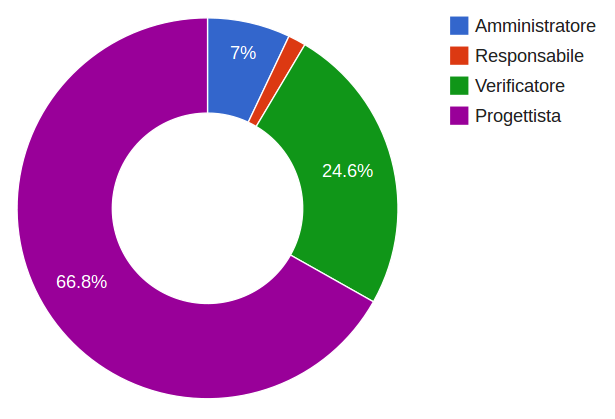
\includegraphics[scale=0.35]{5-2-1.png}
\caption{Ore per ruolo, fase di Progettazione architetturale\label{fig:nome}}
\end{figure}

\begin{figure}[H]
\centering
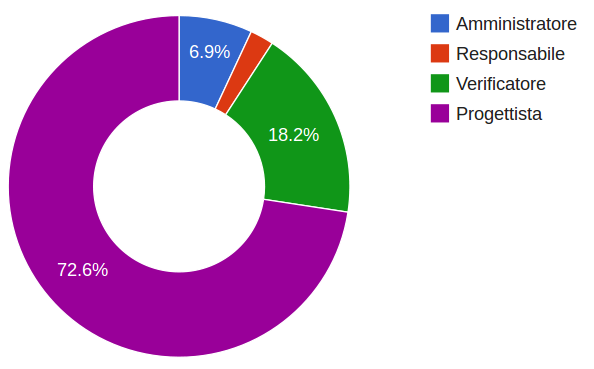
\includegraphics[scale=0.4]{5-2-2.png}
\caption{Costo per ruolo, fase di Progettazione architetturale\label{fig:nome}}
\end{figure}

\subsection{Progettazione di dettaglio e codifica}

Nella fase di Progettazione di dettaglio e codifica le ore per ogni ruolo sono state cosi suddivise:

\begin{table}[H]
	\centering
	\begin{tabular}{ l c c }
	\textbf{Ruolo} & \textbf{Ore} & \textbf{Costo} \\
	\hline
	Amministratore & 26 & 520 €\\
	Analista & 0 & 0 \\
	Progettista & 126 & 2772 €\\
	Programmatore & 160 & 2400 €\\
	Responsabile & 10 & 300 €\\
	Verificatore & 110 & 1650 €\\
	\hline
	\textbf{Totale} & 432 & 7642 €\\
	\hline
	\end{tabular}
	\caption{Ore e costo per ruolo, fase di Progettazione di dettaglio e codifica}
	\end{table}

I seguenti grafici mostrano il peso orario e di costo di ogni ruolo in questa fase.

\begin{figure}[H]
\centering
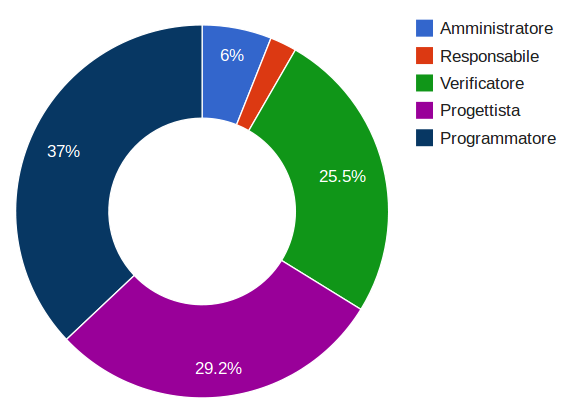
\includegraphics[scale=0.35]{5-3-1.png}
\caption{Ore per ruolo, fase di Progettazione di dettaglio e codifica\label{fig:nome}}
\end{figure}

\begin{figure}[H]
\centering
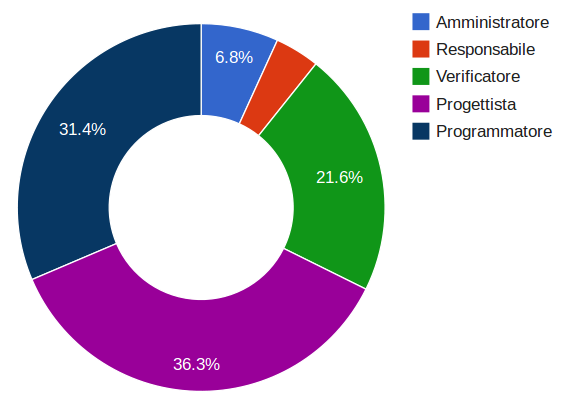
\includegraphics[scale=0.35]{5-3-2.png}
\caption{Costo per ruolo, fase di Progettazione di dettaglio e codifica\label{fig:nome}}
\end{figure}

\subsection{Validazione}

Nella fase di Validazione le ore per ogni ruolo sono state cosi suddivise:

\begin{table}[H]
	\centering
	\begin{tabular}{ l c c }
	\textbf{Ruolo} & \textbf{Ore} & \textbf{Costo} \\
	\hline
	Amministratore & 11 & 220 €\\
	Analista & 0 & 0 €\\
	Progettista & 19 & 418 €\\
	Programmatore & 16 & 240 €\\
	Responsabile & 9 & 270 €\\
	Verificatore & 33 & 495 €\\
	\hline
	\textbf{Totale} & 88 & 1643 €\\
	\hline
	\end{tabular}
	\caption{Ore e costo per ruolo, fase di Validazione}
	\end{table}

I seguenti grafici mostrano il peso orario e di costo di ogni ruolo in questa fase.

\begin{figure}[H]
\centering
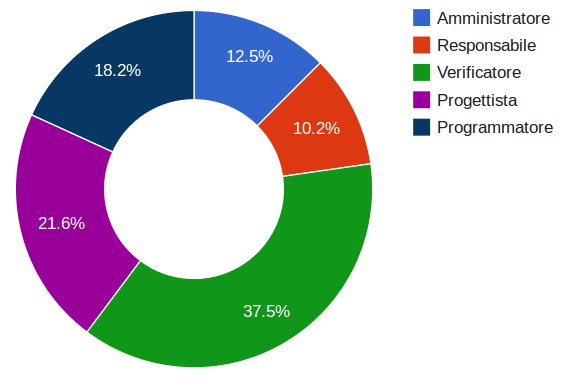
\includegraphics[scale=0.35]{5-4-1.png}
\caption{Ore per ruolo, fase di Validazione\label{fig:nome}}
\end{figure}

\begin{figure}[H]
\centering
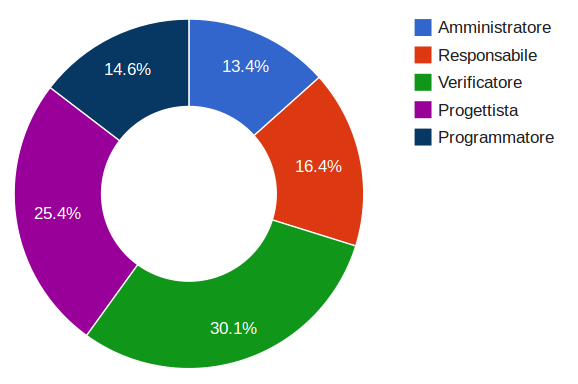
\includegraphics[scale=0.35]{5-4-2.png}
\caption{Costo per ruolo, fase di Validazione\label{fig:nome}}
\end{figure}

\subsection{Totale}

In totale le ore per ogni ruolo sono state cosi suddivise:

\begin{table}[H]
	\centering
	\begin{tabular}{ l c c }
	\textbf{Ruolo} & \textbf{Ore} & \textbf{Costo} \\
	\hline
	Amministratore & 51 & 1020 €\\
	Analista & 0 & 0 €\\
	Progettista & 278 & 6116 €\\
	Programmatore & 176 & 2640 €\\
	Responsabile & 22 & 660 €\\
	Verificatore & 192 & 2880 €\\
	\hline
	\textbf{Totale} & 719 & 13316 €\\
	\hline
	\end{tabular}
	\caption{Ore e costo per ruolo, riassunto progetto}
	\end{table}

I seguenti grafici mostrano il peso orario e di costo di ogni ruolo durante tutto lo svolgimento del progetto, esclusa la fase di Analisi dei requisiti.

\begin{figure}[H]
\centering
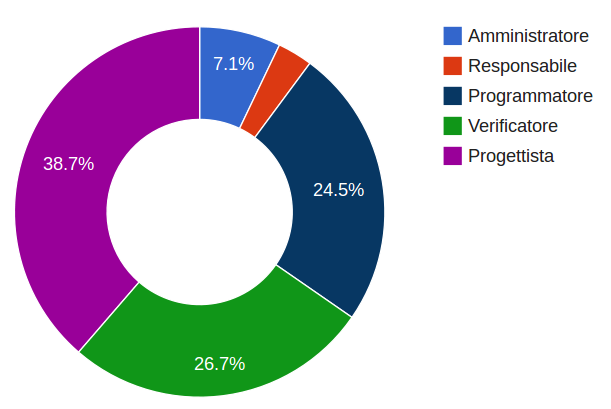
\includegraphics[scale=0.35]{5-5-1.png}
\caption{Ore per ruolo\label{fig:nome}}
\end{figure}

\begin{figure}[H]
\centering
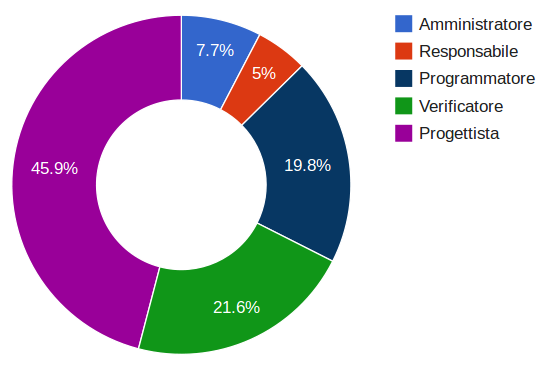
\includegraphics[scale=0.4]{5-5-2.png}
\caption{Costo per ruolo\label{fig:nome}}
\end{figure}
